\documentclass[fleqn, a4paper, 11pt, oneside]{amsart}
%\usepackage[top = 2cm, bottom = 1cm, left = 1cm, right = 1cm]{geometry}
\usepackage{exsheets, tasks}
\usepackage{amsmath, amssymb, amsthm} %standard AMS packages
\usepackage{marginnote} %marginnotes
\usepackage{gensymb} %miscellaneous symbols
\usepackage{commath} %differential symbols
\usepackage{xcolor} %colours
\usepackage{cancel} %cancelling terms
\usepackage[free-standing-units, space-before-unit]{siunitx} %formatting units
	\sisetup
	{
		per-mode=fraction,
		fraction-function=\frac
	}
\usepackage{tikz, pgfplots} %diagrams
\usetikzlibrary{calc, hobby, patterns, intersections, decorations.markings}
\usepackage{graphicx} %inserting graphics
\usepackage{hyperref} %hyperlinks
\usepackage{datetime} %date and time
\usepackage{ulem} %underline for \emph{}
\usepackage{xfrac} %inline fractions
\usepackage{enumerate,enumitem} %numbered lists
\usepackage{float} %inserting floats
\usepackage{circuitikz}[american voltages, american currents] %circuit diagrams
\usepackage[utf8]{inputenc}
\usepackage{booktabs}

\newcommand\numberthis{\addtocounter{equation}{1}\tag{\theequation}} %adds numbers to specific equations in non-numbered list of equations

\newcommand{\AxisRotator}[1][rotate=0]{
	\tikz [x=0.25cm,y=0.60cm,line width=.2ex,-stealth,#1] \draw (0,0) arc (-150:150:1 and 1);%
} %rotation symbols on axes

\theoremstyle{definition}
\newtheorem{example}{Example}
\newtheorem{definition}{Definition}

\theoremstyle{theorem}
\newtheorem{theorem}{Theorem}

\newcommand{\curl}{\mathrm{curl\,}}

\makeatletter
\@addtoreset{section}{part} %resets section numbers in new part
\makeatother

\renewcommand{\thesubsection}{(\arabic{subsection})}
\renewcommand{\thesection}{(\arabic{section})}

\renewcommand{\emph}{\uline}

\renewcommand{\tilde}{\widetilde}

%section headings on left
\makeatletter
\def\specialsection{\@startsection{section}{1}%
	\z@{\linespacing\@plus\linespacing}{.5\linespacing}%
	%  {\normalfont\centering}}% DELETED
	{\normalfont}}% NEW
\def\section{\@startsection{section}{1}%
	\z@{.7\linespacing\@plus\linespacing}{.5\linespacing}%
	%  {\normalfont\scshape\centering}}% DELETED
	{\normalfont\scshape}}% NEW
\makeatother

%forces newline after subsection
\makeatletter
\def\subsection{\@startsection{subsection}{3}%
	\z@{.5\linespacing\@plus.7\linespacing}{.1\linespacing}%
	{\normalfont\itshape}}
\makeatother

\settasks{counter-format = tsk[1].}

\SetupExSheets{solution/print = true}

%opening
\title{Quantum and Solid State Physics : Assignment 7}
\author
{
	Aakash Jog\\
	ID : 989323563
}
\date{\formatdate{3}{12}{2015}}

\begin{document}

\tikzset{->-/.style={decoration={
  markings,
  mark=at position #1 with {\arrow{>}}},postaction={decorate}}}

\maketitle
%\setlength{\mathindent}{0pt}

\begin{question}
	Consider a semiconductor sample with both an electric field $\overrightarrow{E}$ and carrier concentration gradient.
	Shown below is the equilibrium band diagram across the length of the sample, and also the carrier concentrations, $\log n$, $\log p$, as functions of position across the sample.
	\begin{figure}[H]
		\centering
		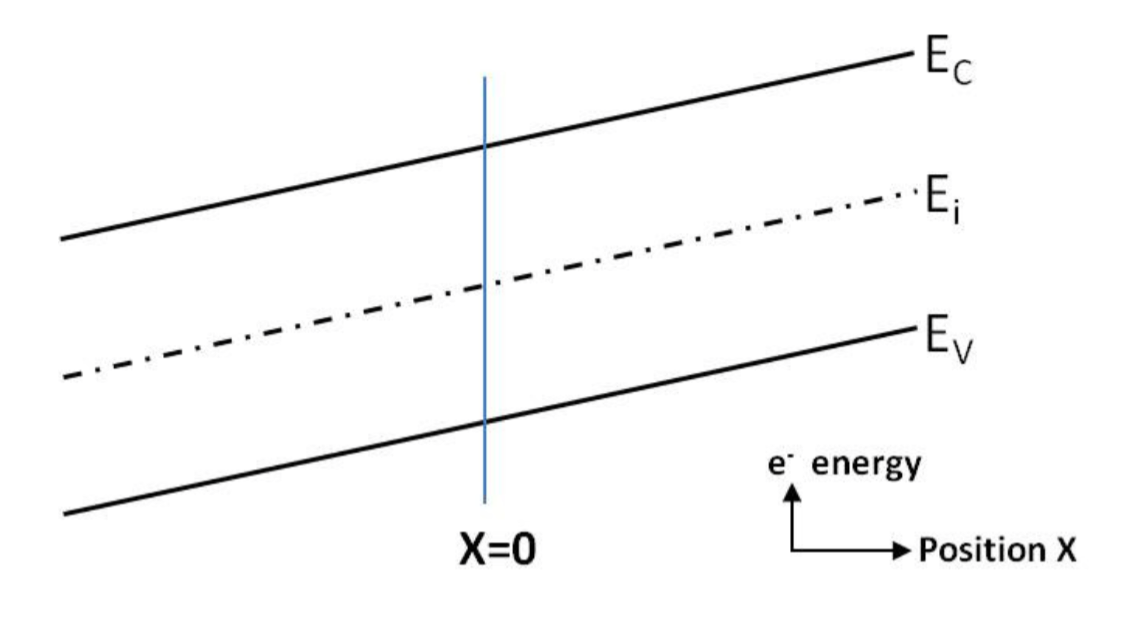
\includegraphics[width = 0.5\textwidth]{fig1.png}
	\end{figure}
	\begin{figure}[H]
		\centering
		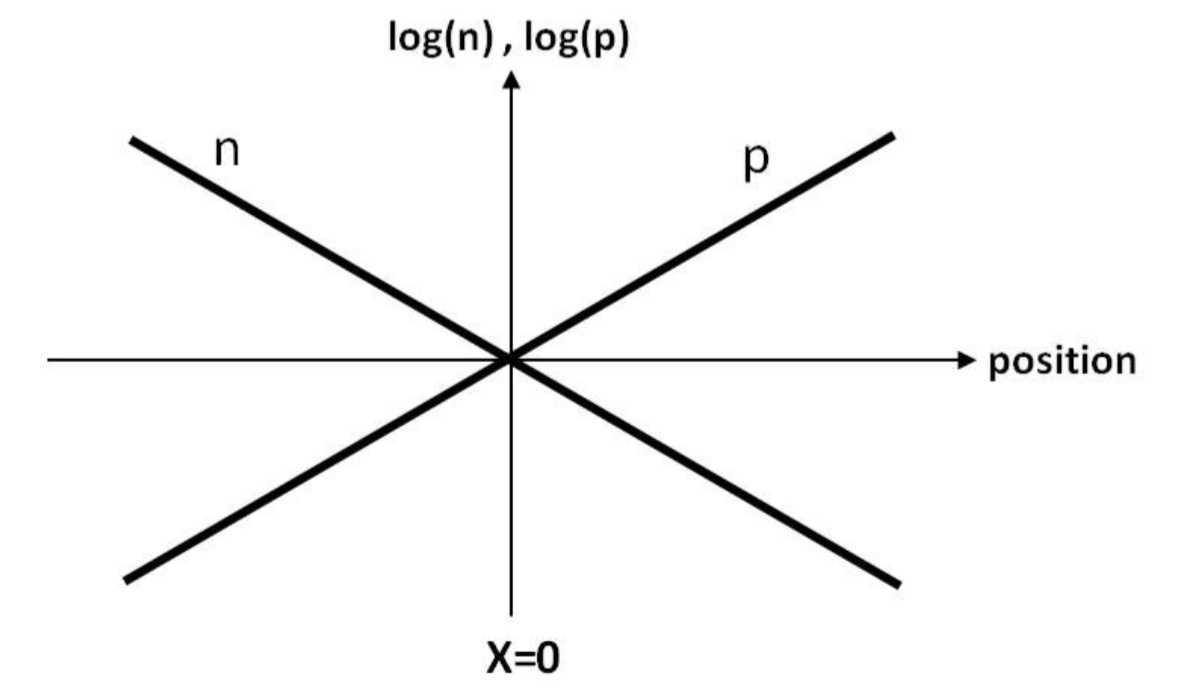
\includegraphics[width = 0.5\textwidth]{fig2.png}
	\end{figure}
	\begin{enumerate}
		\item
			What is the direction of the electric field?
			Is $\overrightarrow{E}$ constant, with respect to $x$, or dependent on $x$?
			Choose the correct answer below.
			\begin{enumerate}
				\item $\rightarrow$, constant
				\item $\rightarrow$, position dependent
				\item $\leftarrow$, constant
				\item $\leftarrow$, position dependent
			\end{enumerate}
		\item
			Indicate with arrows, the correct direction of electron and hole flow in the sample due to both diffusion and drift, and the correct direction of the corresponding current densities.
	\end{enumerate}
\end{question}

\begin{solution}
	\begin{enumerate}[leftmargin=*]
		\item
			The electric field is directed $\rightarrow$, and is constant.
		\item
			\begin{table}[H]
				\centering
				\begin{tabular}{l l l l}
					\toprule
					Direction of electron drift & $\leftarrow$ & $J_{\text{drift}_n}$ & $\rightarrow$\\
					Direction of electron diffusion & $\rightarrow$ & $J_{\text{diffusion}_n}$ & $\leftarrow$\\
					Direction of hole drift & $\rightarrow$ & $J_{\text{drift}_p}$ & $\rightarrow$\\
					Direction of hole diffusion & $\leftarrow$ & $J_{\text{diffusion}_p}$ & $\leftarrow$\\
					\bottomrule
				\end{tabular}
			\end{table}
	\end{enumerate}
\end{solution}

\begin{question}
	Shown below is the electron mobility dependence on temperature for a sample of Silicon.
	\begin{figure}[H]
		\centering
		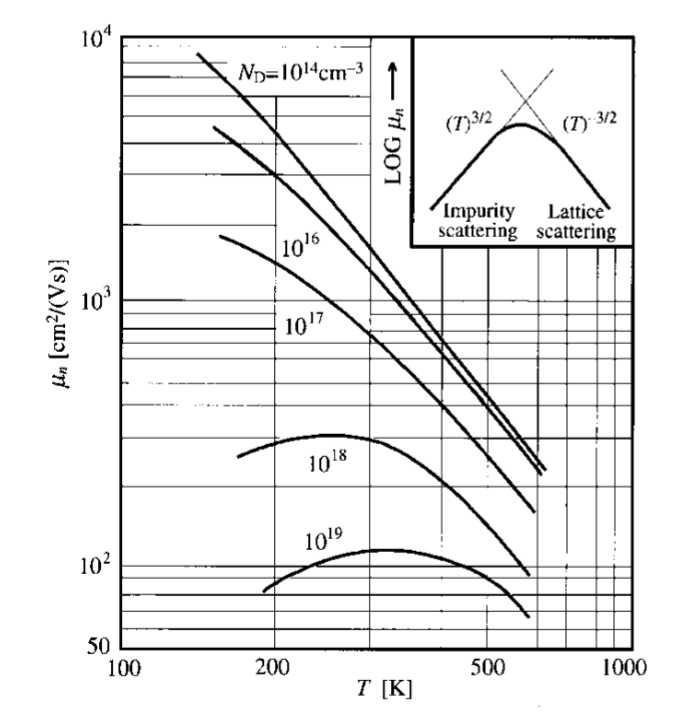
\includegraphics[width = 0.5\textwidth]{fig3.png}
	\end{figure}
	Calculate the resistivity $\rho$ of this sample of Silicon at 300 \kelvin, when it is doped with $10^{16}$ Phosphorus atoms per \si{\centi\metre\cubed}, and $10^{14}$ Boron atoms per \si{\centi\metre\cubed}.
\end{question}

\begin{solution}
	As the concentration of Phosphorus atoms is more than that of Boron atoms, the material is N-type.\\
	Therefore,
	\begin{align*}
		\rho & = \frac{1}{q \mu_n n}                                                                                                                                                       \\
                     & = \frac{1}{q \mu_n}                                                                                                                                                         \\
                     & = \frac{1}{\left( 1.6 \times 10^{19} \coulomb \right) \left( 10^3 \si{\centi\metre\squared\per\volt\per\second} \right) \left( 10^{16} \si{\per\centi\metre\cubed} \right)} \\
                     & = 0.625 \si{\ohm\centi\metre}
	\end{align*}
\end{solution}

\begin{question}
	A free particle has the following initial wave function, i.e. at $t = 0$,
	\begin{align*}
		\psi(x,0) & = A e^{-a |x|}
	\end{align*}
	where $A$ and $a$ are positive and real constants.
	\begin{enumerate}
		\item
			Find $A$.
		\item
			Find $\tilde{\psi}(k)$.
			Remember that
			\begin{align*}
				\psi(x,0) & = \frac{1}{\sqrt{2 \pi}} \int\limits_{-\infty}^{\infty} \tilde{\psi}(k) e^{i k x} \dif k
			\end{align*}
			Also, use your knowledge of even and odd functions to help you solve the integral.
		\item
			Construct $\psi(x,t)$.
			Your answer should simply show the integral.
		\item
			Consider a case where $a$ is very small.
			What can you say about the uncertainty in position and momentum for the particle at $t = 0$, described by the wave function $\psi(x,0)$?
		\item
			Consider a case where $a$ is very large.
			What can you say about the uncertainty in position and momentum for the particle at $t = 0$, described by the wave function $\psi(x,0)$?
	\end{enumerate}
\end{question}

\begin{solution}
	\begin{enumerate}[leftmargin=*]
		\item
			\begin{align*}
				1            & = \int\limits_{-\infty}^{\infty} \left| \psi(x,0) \right|^2 \dif x \\
                                             & = \int\limits_{-\infty}^{\infty} A^2 e^{-2 a |x|} \dif x           \\
                                             & = 2 A^2 \int\limits_{0}^{\infty} e^{-2 a x} \dif x                 \\
                                             & = 2 A^2 \left. \frac{e^{-2 a x}}{-2 a} \right|_{0}^{\infty}        \\
                                             & = 2 A^2 \left( 0 - \frac{1}{2 a} \right)                           \\
                                             & = \frac{2 A^2}{2 a}                                                \\
				\therefore A & = \sqrt{a}
			\end{align*}
		\item
			\begin{align*}
				\tilde{\psi}(k) & = \frac{1}{\sqrt{2 \pi}} \int\limits_{-\infty}^{\infty} \psi(x,0) e^{-i k x} \dif x           \\
                                                & = \frac{1}{\sqrt{2 \pi}} \int\limits_{-\infty}^{\infty} \sqrt{a} e^{-a |x|} e^{-i k x} \dif x \\
                                                & = \sqrt{\frac{2 a}{\pi}} \frac{a}{a^2 + k^2}
			\end{align*}
		\item
			\begin{align*}
				\psi(x,t) & = \frac{1}{\sqrt{2 \pi}} \int\limits_{-\infty}^{\infty} \tilde{\psi}(k) e^{i k x} e^{-\frac{i E t}{\hbar}} \dif k \\
                                          & = \frac{a^{\frac{3}{2}}}{\pi} \int\limits_{-\infty}^{\infty} \frac{e^{i k x} e^{-\frac{i k^2 \hbar}{2 m} t}}{a^2 + k^2} \dif k
			\end{align*}
		\item
			If $a$ is very small, $\psi(x,0)$ is almost constant.
			Hence, $\sigma_x$ is high, and $\sigma_p$ is low.
		\item
			If $a$ is very large, $\psi(x,0)$ is large.
			Hence, $\sigma_x$ is low, and $\sigma_p$ is high.
	\end{enumerate}
\end{solution}

\begin{question}
	Consider a case of even potential, such that $V(-x) = V(x)$.
	\begin{enumerate}
		\item
			If $\psi(x)$ is a solution to the time independent Schrödinger equation, what can you say about $\psi(-x)$?
			Hint: Replace $x$ by $-x$ in the Schrödinger equation.
		\item
			Based on the principle of superposition, suggest a way of constructing an even and an odd solution from $\psi(x)$ and $\psi(-x)$.
			Don't forget to normalize.
	\end{enumerate}
\end{question}

\begin{solution}
	\begin{enumerate}[leftmargin=*]
		\item
			\begin{align*}
				-\frac{\hbar^2}{2 m} \dod[2]{\psi(x)}{x} + V(x) \psi(x) & = E \psi(x)
			\end{align*}
			Therefore, replacing $x$ by $-x$,
			\begin{align*}
				-\frac{\hbar^2}{2 m} \dod[2]{\psi(-x)}{x} + V(-x) \psi(-x) & = E \psi(-x)
			\end{align*}
			Therefore, as $V(-x) = V(x)$,
			\begin{align*}
				-\frac{\hbar^2}{2 m} \dod[2]{\psi(-x)}{x} + V(x) \psi(-x) & = E \psi(-x)
			\end{align*}
			Therefore, $\psi(-x)$ is also a solution to the time independent Schrödinger equation.
	\end{enumerate}
\end{solution}

\begin{question}
	Repeat the derivation of the solution to the finite well potential, this time looking only at the odd solutions.
	The general solution in this case is
	\begin{align*}
		\psi(x) &=
			\begin{cases}
				A e^{k x}       & ;\quad x < -a         \\
				F \sin(\beta x) & ;\quad -a \le x \le a \\
				C e^{-k x}      & ;\quad a < x          \\
			\end{cases}
	\end{align*}
	where the potential is defined as
	\begin{align*}
		V(x) &=
			\begin{cases}
				0    & ;\quad x < -a         \\
				-V_0 & ;\quad -a \le x \le a \\
				0    & ;\quad a < x          \\
			\end{cases}
	\end{align*}
	\begin{enumerate}
		\item
			Find the equation linking $k$ and $\beta$.
		\item
			Define $z = \beta a$ and $y = k a$, and draw the two sets of curves.
		\item
			Sketch how we find the allowed states using your results from above.
		\item
			Is there always an allowed odd state?
		\item
			When $V_0$ approaches infinity, describe the allowed energy states in terms of allowed values of $\beta$.
			Verify that your result combined with the similar result we got in class for the even solutions describes the allowed states in an infinite potential well.
	\end{enumerate}
\end{question}

\begin{solution}
	\begin{enumerate}[leftmargin=*]
		\item
			\begin{align*}
				\psi(x) &=
					\begin{cases}
						A e^{k x}       & ;\quad x < -a         \\
						F \sin(\beta x) & ;\quad -a \le x \le a \\
						C e^{-k x}      & ;\quad a < x          \\
					\end{cases}
			\end{align*}
			As $\psi$ is continuous at the boundaries,
			\begin{align*}
				A e^{-k a}      & = F \sin(-\beta a) \\
				F \sin(\beta a) & = C e^{-k a}
			\end{align*}
			Therefore,
			\begin{align*}
				A & = -C
			\end{align*}
			As $\psi'$ is continuous at the boundaries,
			\begin{align*}
				A k e^{-k a}          & = F \beta \cos(-\beta a) \\
				F \beta \cos(\beta a) & = -C k e^{-k a}
			\end{align*}
			Therefore,
			\begin{align*}
				-k & = \beta \cot(\beta a)
			\end{align*}
		\item
			Let
			\begin{align*}
				z & = \beta a \\
				y & = k a
			\end{align*}
			Therefore,
			\begin{align*}
				y         & = -z \cot z \\
				y^2 + z^2 & = {R_0}^2
			\end{align*}
			Therefore,
			\begin{figure}[H]
				\centering
				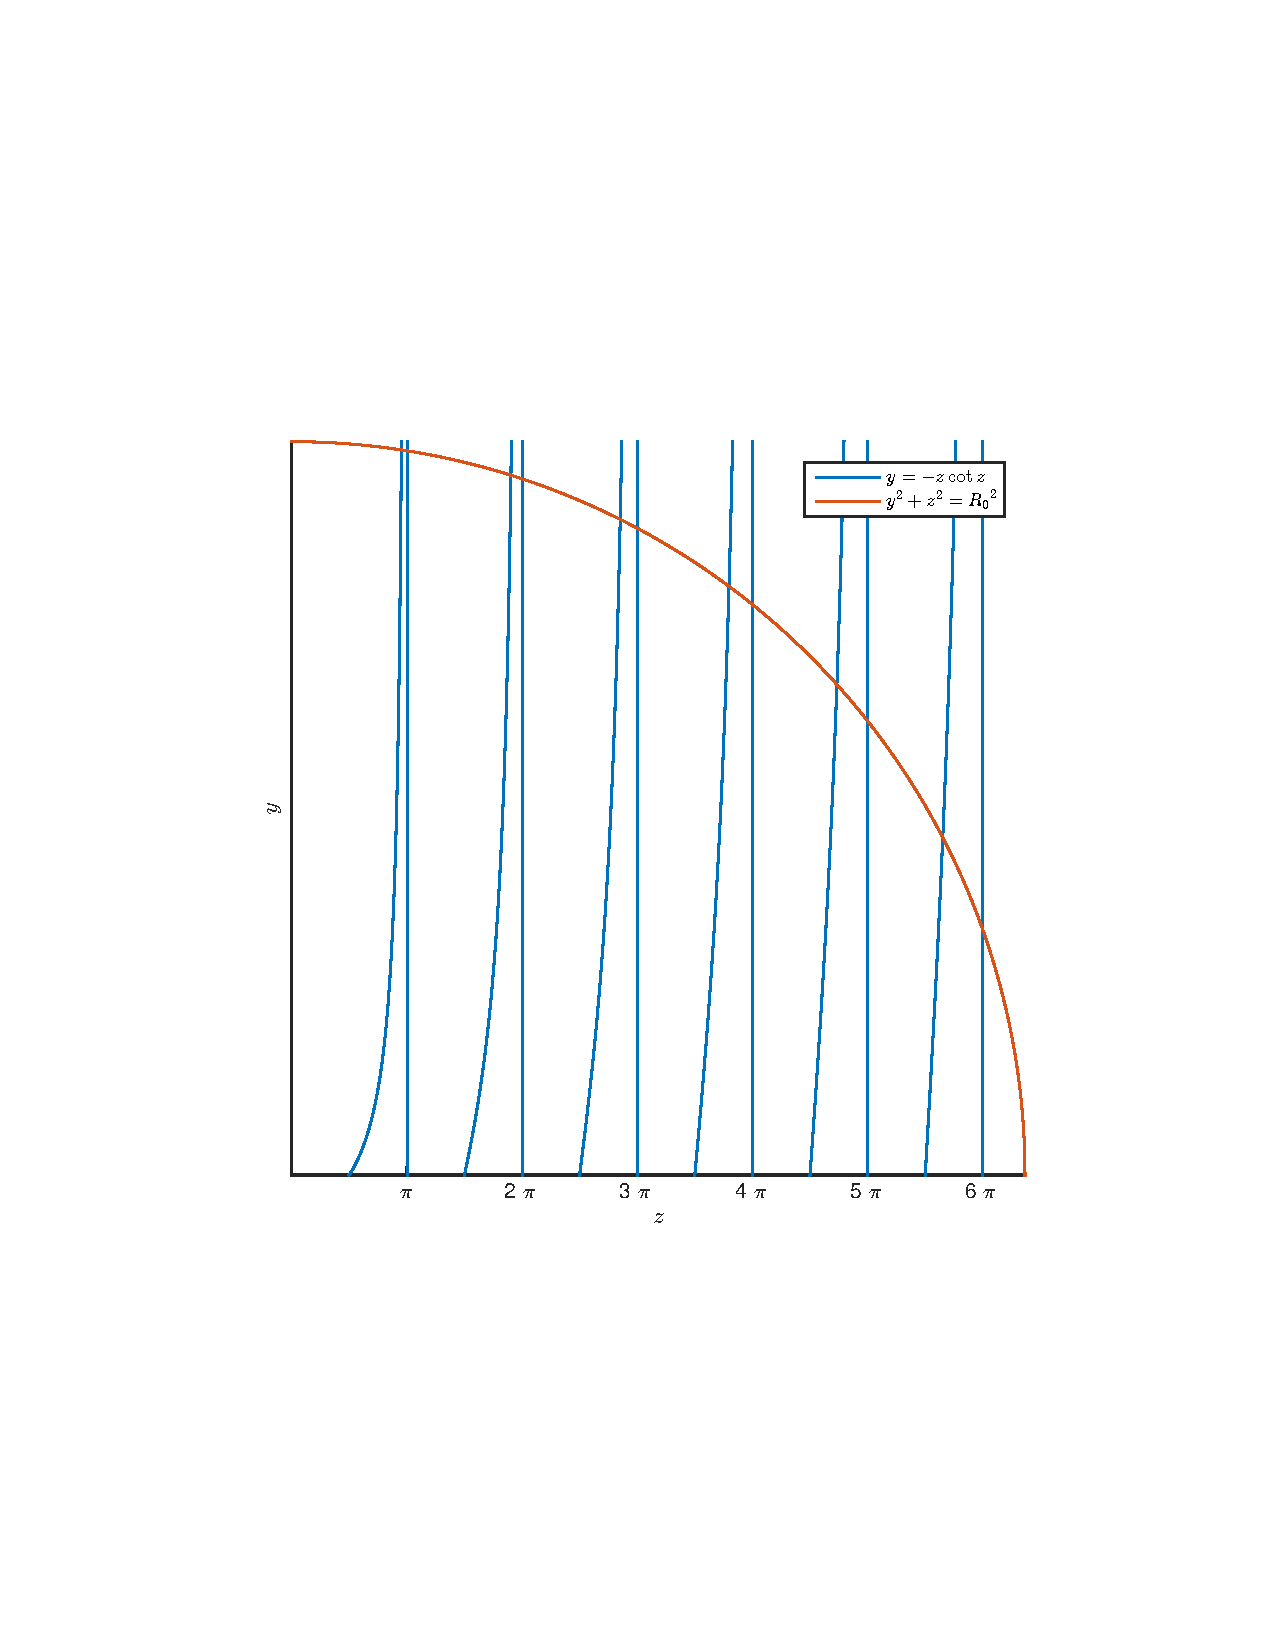
\includegraphics[width = \textwidth]{plot1.pdf}
			\end{figure}
		\item
			
		\item
			If $R_0 < \frac{\pi}{2}$, the curves do not intersect, and there is no allowed odd state.
		\item
			If $V_0 \to \infty$, $R_0 \to \infty$,
			\begin{align*}
				z & = n \pi
			\end{align*}
			where $n \in \mathbb{N}$.\\
			Therefore,
			\begin{align*}
				\beta_n & = \frac{n \pi}{2 a}
			\end{align*}
			For an infinite potential well,
			\begin{align*}
				k_n & = \frac{n \pi}{2 a}
			\end{align*}
			Therefore, this is consistent with the result from class.
	\end{enumerate}
\end{solution}

\end{document}
